% Task 7 — Multi-Tier Integration
% Northeast Megaregion Freight Network Design
% Tonnage figures are in thousand short tons (ktons); capacities are in square feet (sf).

\section{Task 7 --- Multi-Tier Integration}

Task~7 assembles the outputs of Tasks~2, 5, and~6 into a single hierarchical freight
network spanning external interfaces, regional hubs, gateway hubs, freight regions, and
freight areas. No new optimisation is introduced at this stage. The work instead
standardises node identifiers, reconciles schemas across tiers, and defines the full edge
catalog used for visualisation and downstream flow assignment. The integrated design
contains \textbf{391 nodes} and \textbf{584 edges}, connecting 29 interface nodes to
50 regional hubs and 312 gateway hubs across 132 freight areas.

\subsection{Unified Node Catalog}

The node catalog is defined as the union of three disjoint sets:

\begin{equation}
  N = N_{\text{RH}} \cup N_{\text{GW}} \cup N_{\text{IF}},
  \qquad
  |N| = 50 + 312 + 29 = 391
  \label{eq:task7-nodes}
\end{equation}

where $N_{\text{RH}}$ is the Task~5 regional-hub set, $N_{\text{GW}}$ is the Task~6
gateway-hub set, and $N_{\text{IF}}$ is the Task~2 interface-node set. Stable
\texttt{node\_id} values preserve tier identity by construction:
\texttt{RH\_\{candidate\_id\}} for regional hubs, \texttt{GW\_\{candidate\_id\}} for
gateways, and \texttt{IF\_\{slug\}} for interface nodes. This convention ensures that
all downstream joins can be performed without ambiguous cross-tier keys.

Regional-hub records inherit the Task~5 facility coordinates, capacities, and
\texttt{region\_id} fields directly. Gateway-hub records inherit the Task~6 facility
fields and attach the parent \texttt{area\_id}. Interface nodes carry no warehouse
capacity; instead, they retain the Task~2 allocated 2025/2030 tonnage after unit
normalisation into ktons. Table~\ref{tab:task7-nodes} summarises the integrated node
inventory.

\begin{table}[htbp]
  \centering
  \caption{Unified node catalog summary by tier and class.}
  \label{tab:task7-nodes}
  \begin{tabular}{lrrl}
    \toprule
    Node class & Count & Tier & Key attribute summary \\
    \midrule
    Regional hubs & 50 & 1 & 285{,}146--500{,}000~sf capacity (median 449{,}340~sf) \\
    Gateway hubs & 312 & 2 & 185{,}432--500{,}000~sf capacity (median 350{,}381~sf) \\
    Interface --- global & 9 & 3 & 519{,}652~ktons in 2025 \\
    Interface --- continental & 8 & 3 & 61{,}248~ktons in 2025 \\
    Interface --- national & 12 & 3 & 213{,}438~ktons in 2025 \\
    \midrule
    \textbf{Total} & \textbf{391} & --- & \textbf{794{,}338~ktons at the interface tier} \\
    \bottomrule
  \end{tabular}
\end{table}

The interface tier is dominated by the global class, which contributes 65.4\% of
all interface throughput in 2025. John F. Kennedy International Airport alone carries
236{,}426~ktons, exceeding the full continental-interface total. This concentration is
important for the integrated design because it implies that a small number of boundary
gateways inject a large share of megaregional freight into the regional backbone.

\subsection{Unified Edge Catalog and Validation}

The edge catalog combines four structurally distinct link sets:

\begin{equation}
  E = E_{\text{HH}} \cup E_{\text{GH}} \cup E_{\text{AA}} \cup E_{\text{IH}},
  \qquad
  |E| = 133 + 329 + 93 + 29 = 584
  \label{eq:task7-edges}
\end{equation}

where $E_{\text{HH}}$ denotes regional hub-to-hub links from Task~5,
$E_{\text{GH}}$ gateway-to-hub links from Task~6,
$E_{\text{AA}}$ inter-area links represented through the largest gateway in each area,
and $E_{\text{IH}}$ interface-to-hub connectors. Interface nodes are attached to the
regional tier by a nearest-hub assignment:

\begin{equation}
  h^\star(i) = \arg\min_{h \in N_{\text{RH}}} d(i,h)
  \label{eq:task7-nearest}
\end{equation}

using Euclidean distance in the common projected CRS. This rule gives each interface
node exactly one inbound connection to the megaregional backbone while preserving a
transparent physical interpretation.

Table~\ref{tab:task7-edges} summarises the integrated edge inventory.

\begin{table}[htbp]
  \centering
  \caption{Unified edge catalog summary by link type.}
  \label{tab:task7-edges}
  \begin{tabular}{lrrrr}
    \toprule
    Edge type & Count & Directed & Mean distance (mi) & Max distance (mi) \\
    \midrule
    Hub-to-hub & 133 & No & 69.2 & 305.6 \\
    Gateway-to-hub & 329 & Yes & 26.5 & 175.3 \\
    Inter-area & 93 & No & 42.0 & 148.4 \\
    Interface-to-hub & 29 & Yes & 245.4 & 2{,}105.8 \\
    \bottomrule
  \end{tabular}
\end{table}

The directed gateway-to-hub layer is geographically local: links average
26.5~miles and carry area demand loads ranging from 184 to 19{,}766~ktons. The
hub-to-hub backbone is longer-range, averaging 69.2~miles with construction weights from
516 to 51{,}469~ktons. Inter-area links supply lateral redundancy within regions rather
than upward transfer, and therefore sit between these two scales at a mean length of
42.0~miles.

The interface-to-hub links show the strongest scale contrast. Global interfaces attach to
nearby coastal or airport-adjacent regional hubs with a mean connector length of only
10.5~miles, while continental links average 121.7~miles. National interface links average
504.0~miles because they represent external domestic anchors rather than nodes inside the
Northeast footprint; the longest connection is the Los Angeles interface node to its
nearest regional hub at 2{,}105.8~miles. These long connectors are therefore boundary
conditions for the megaregional model, not local drayage movements.

Validation confirms that the assembled topology is internally consistent. No orphan edges
exist: every \texttt{from\_node\_id} and \texttt{to\_node\_id} in \texttt{edges.csv}
matches a node in \texttt{nodes.csv}. Every regional hub participates in at least one
hub-to-hub edge and at least one gateway-to-hub edge, and every interface node appears in
exactly one interface-to-hub edge. The integrated graph is therefore complete enough to
support the Task~8 routing logic without additional manual patching.

\subsection{Integrated Geography and Hierarchy}

Figure~\ref{fig:task7-map} overlays the four link types and all node tiers on the NE
basemap. The resulting pattern is strongly corridor-oriented. Regional hubs form a
coherent blue backbone across the megaregion; gateway hubs densify around the I-95
coastal belt, eastern Pennsylvania, and the Baltimore--Washington corridor; and the
interface nodes anchor the regional structure to major seaports, airports, border
crossings, and high-volume external domestic counties.

\begin{figure}[htbp]
  \centering
  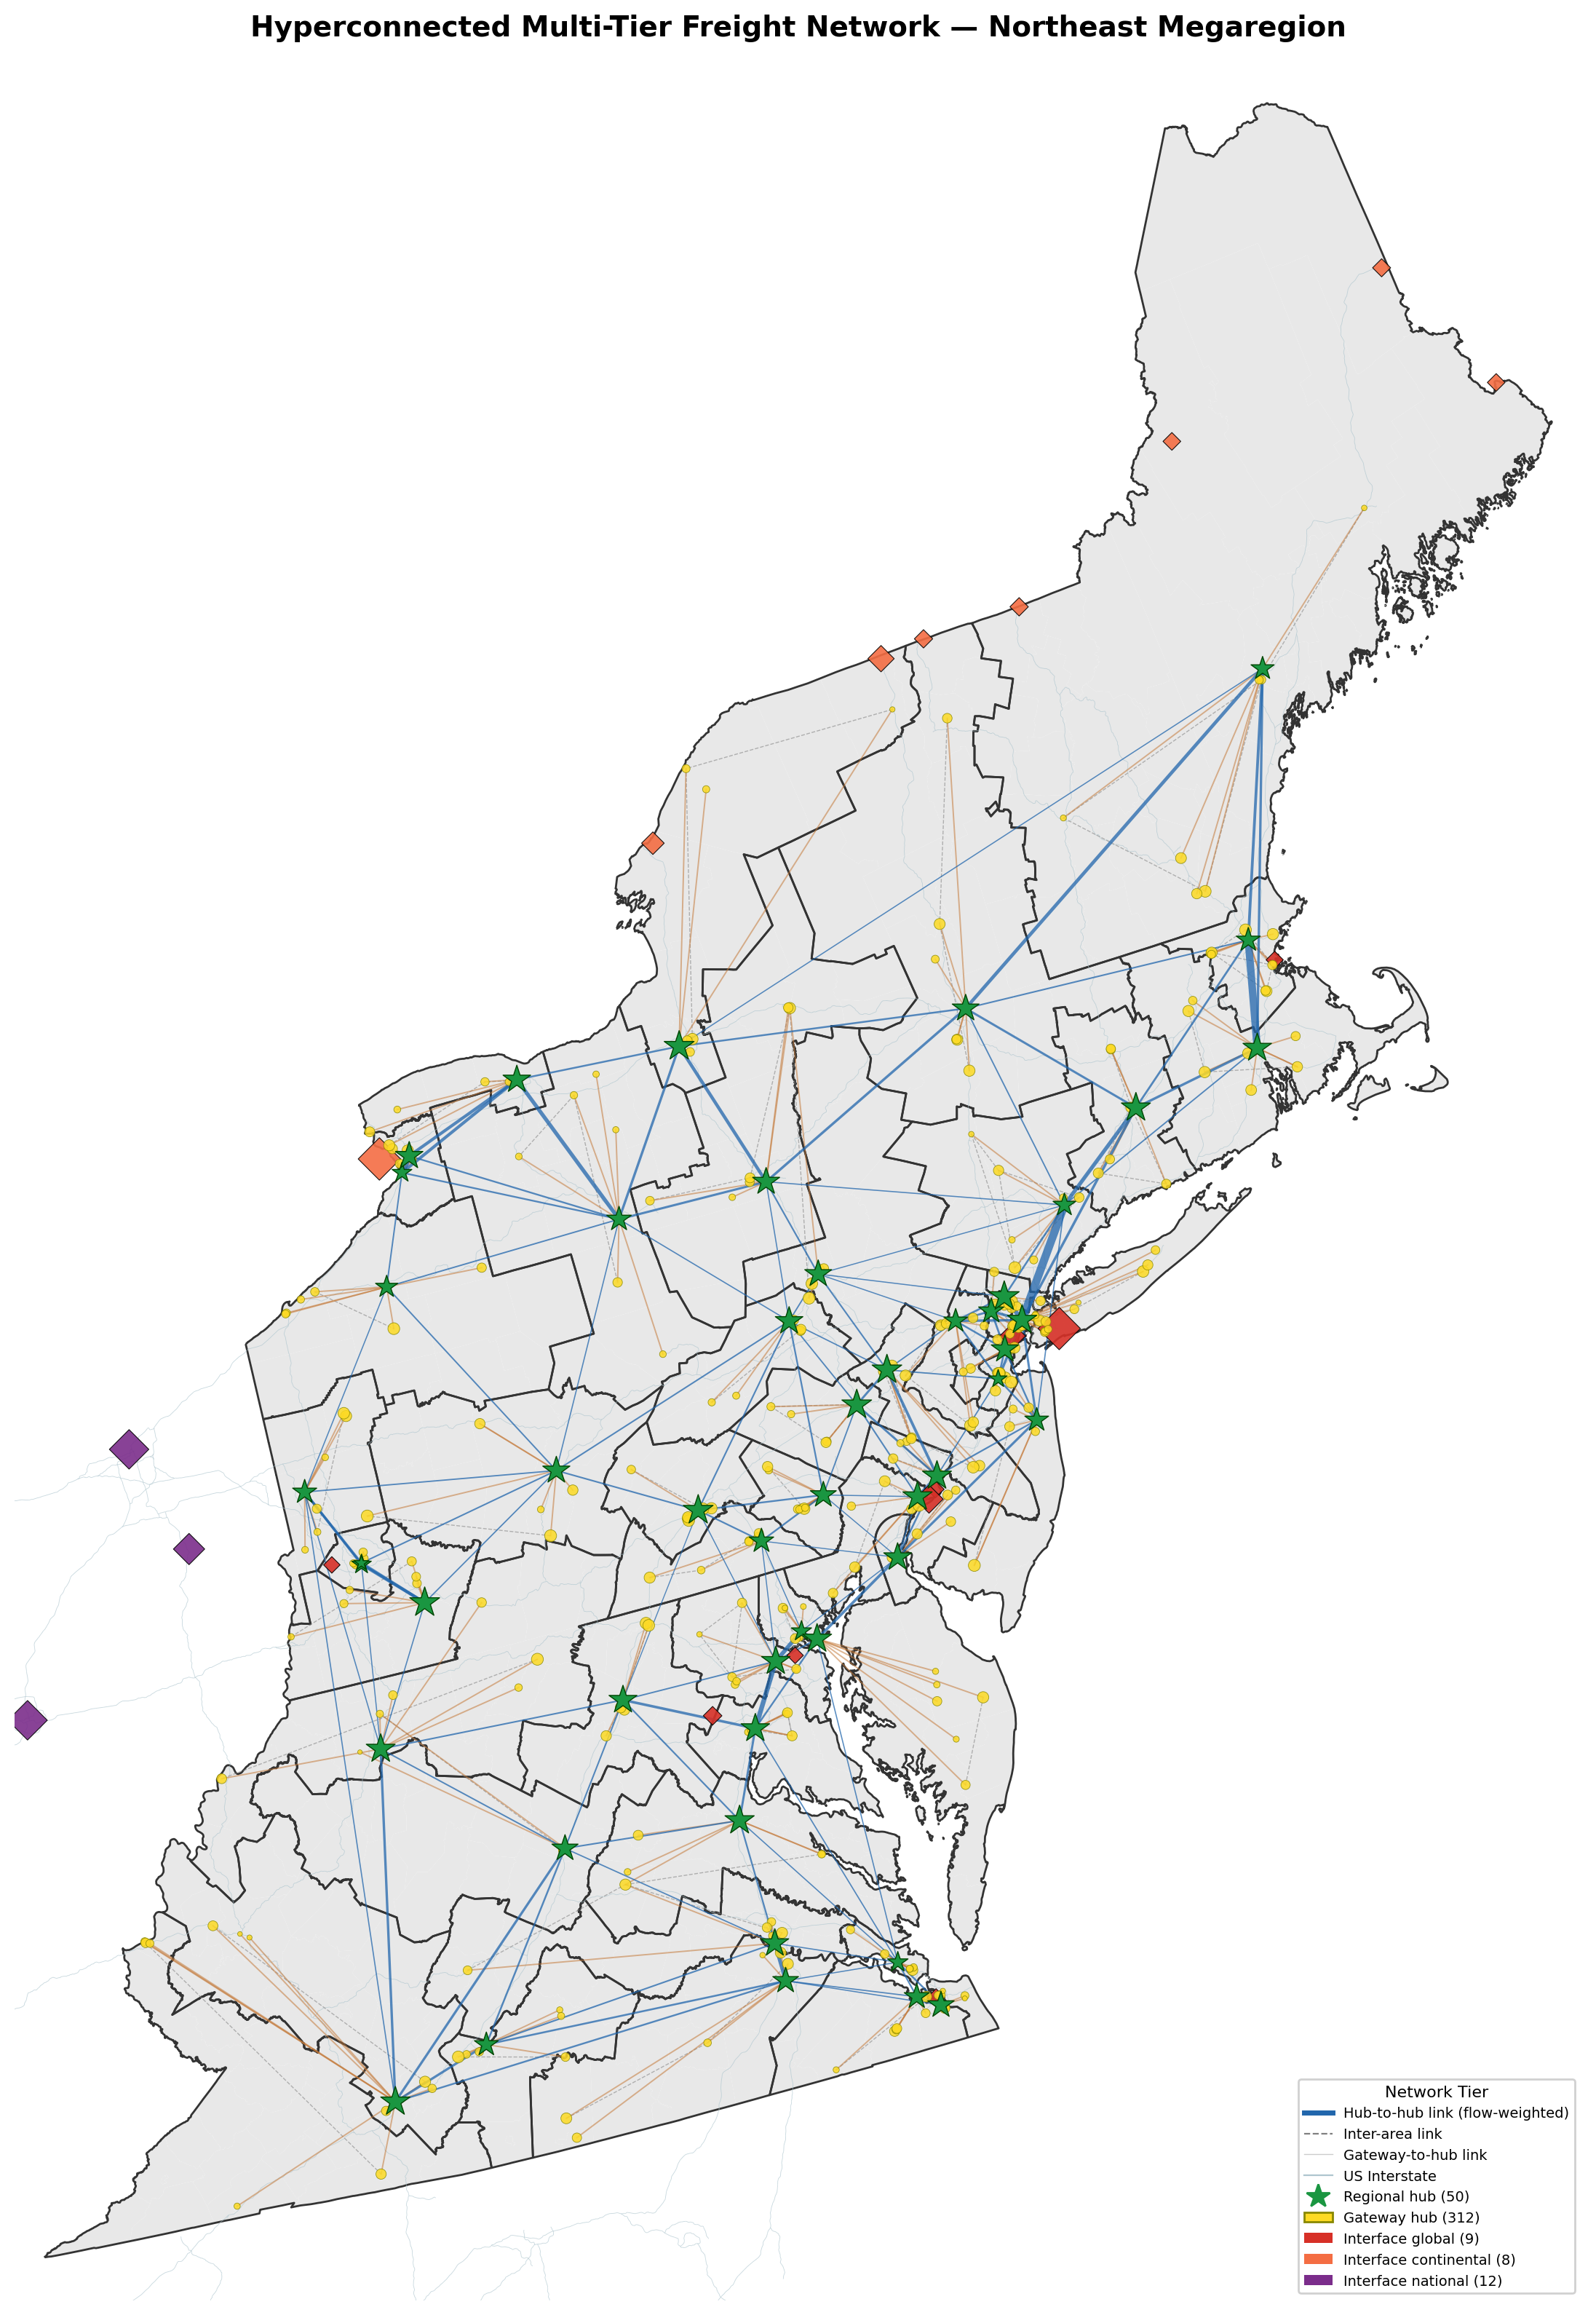
\includegraphics[width=0.84\textwidth,height=0.72\textheight,keepaspectratio]{figures/task7_multitier_map.png}
  \caption{Integrated multi-tier freight network across the Northeast megaregion.
    Thick blue links denote the regional hub backbone, thin amber links connect gateway
    hubs upward to the regional tier, dashed gray links show inter-area connectivity, and
    diamond markers denote global, continental, and national interface nodes. The densest
    concentration of gateway and regional nodes occurs along the I-95 corridor and in the
    New Jersey--eastern Pennsylvania distribution belt.}
  \label{fig:task7-map}
\end{figure}

The map also shows how the structure supports freight movement at three scales. External
flows first enter the network through a compact set of interface connectors, then move
laterally across the regional-hub backbone, and finally disperse through the denser
gateway layer into metropolitan freight areas. This staged topology is precisely the
hierarchical logic requested in the handout: global and national interfaces inject flows
into the megaregion, the regional tier handles cross-megaregion transfer, and the gateway
tier handles access to major urban concentrations.

Figure~\ref{fig:task7-schematic} makes the same logic explicit in non-geographic form.

\begin{figure}[htbp]
  \centering
  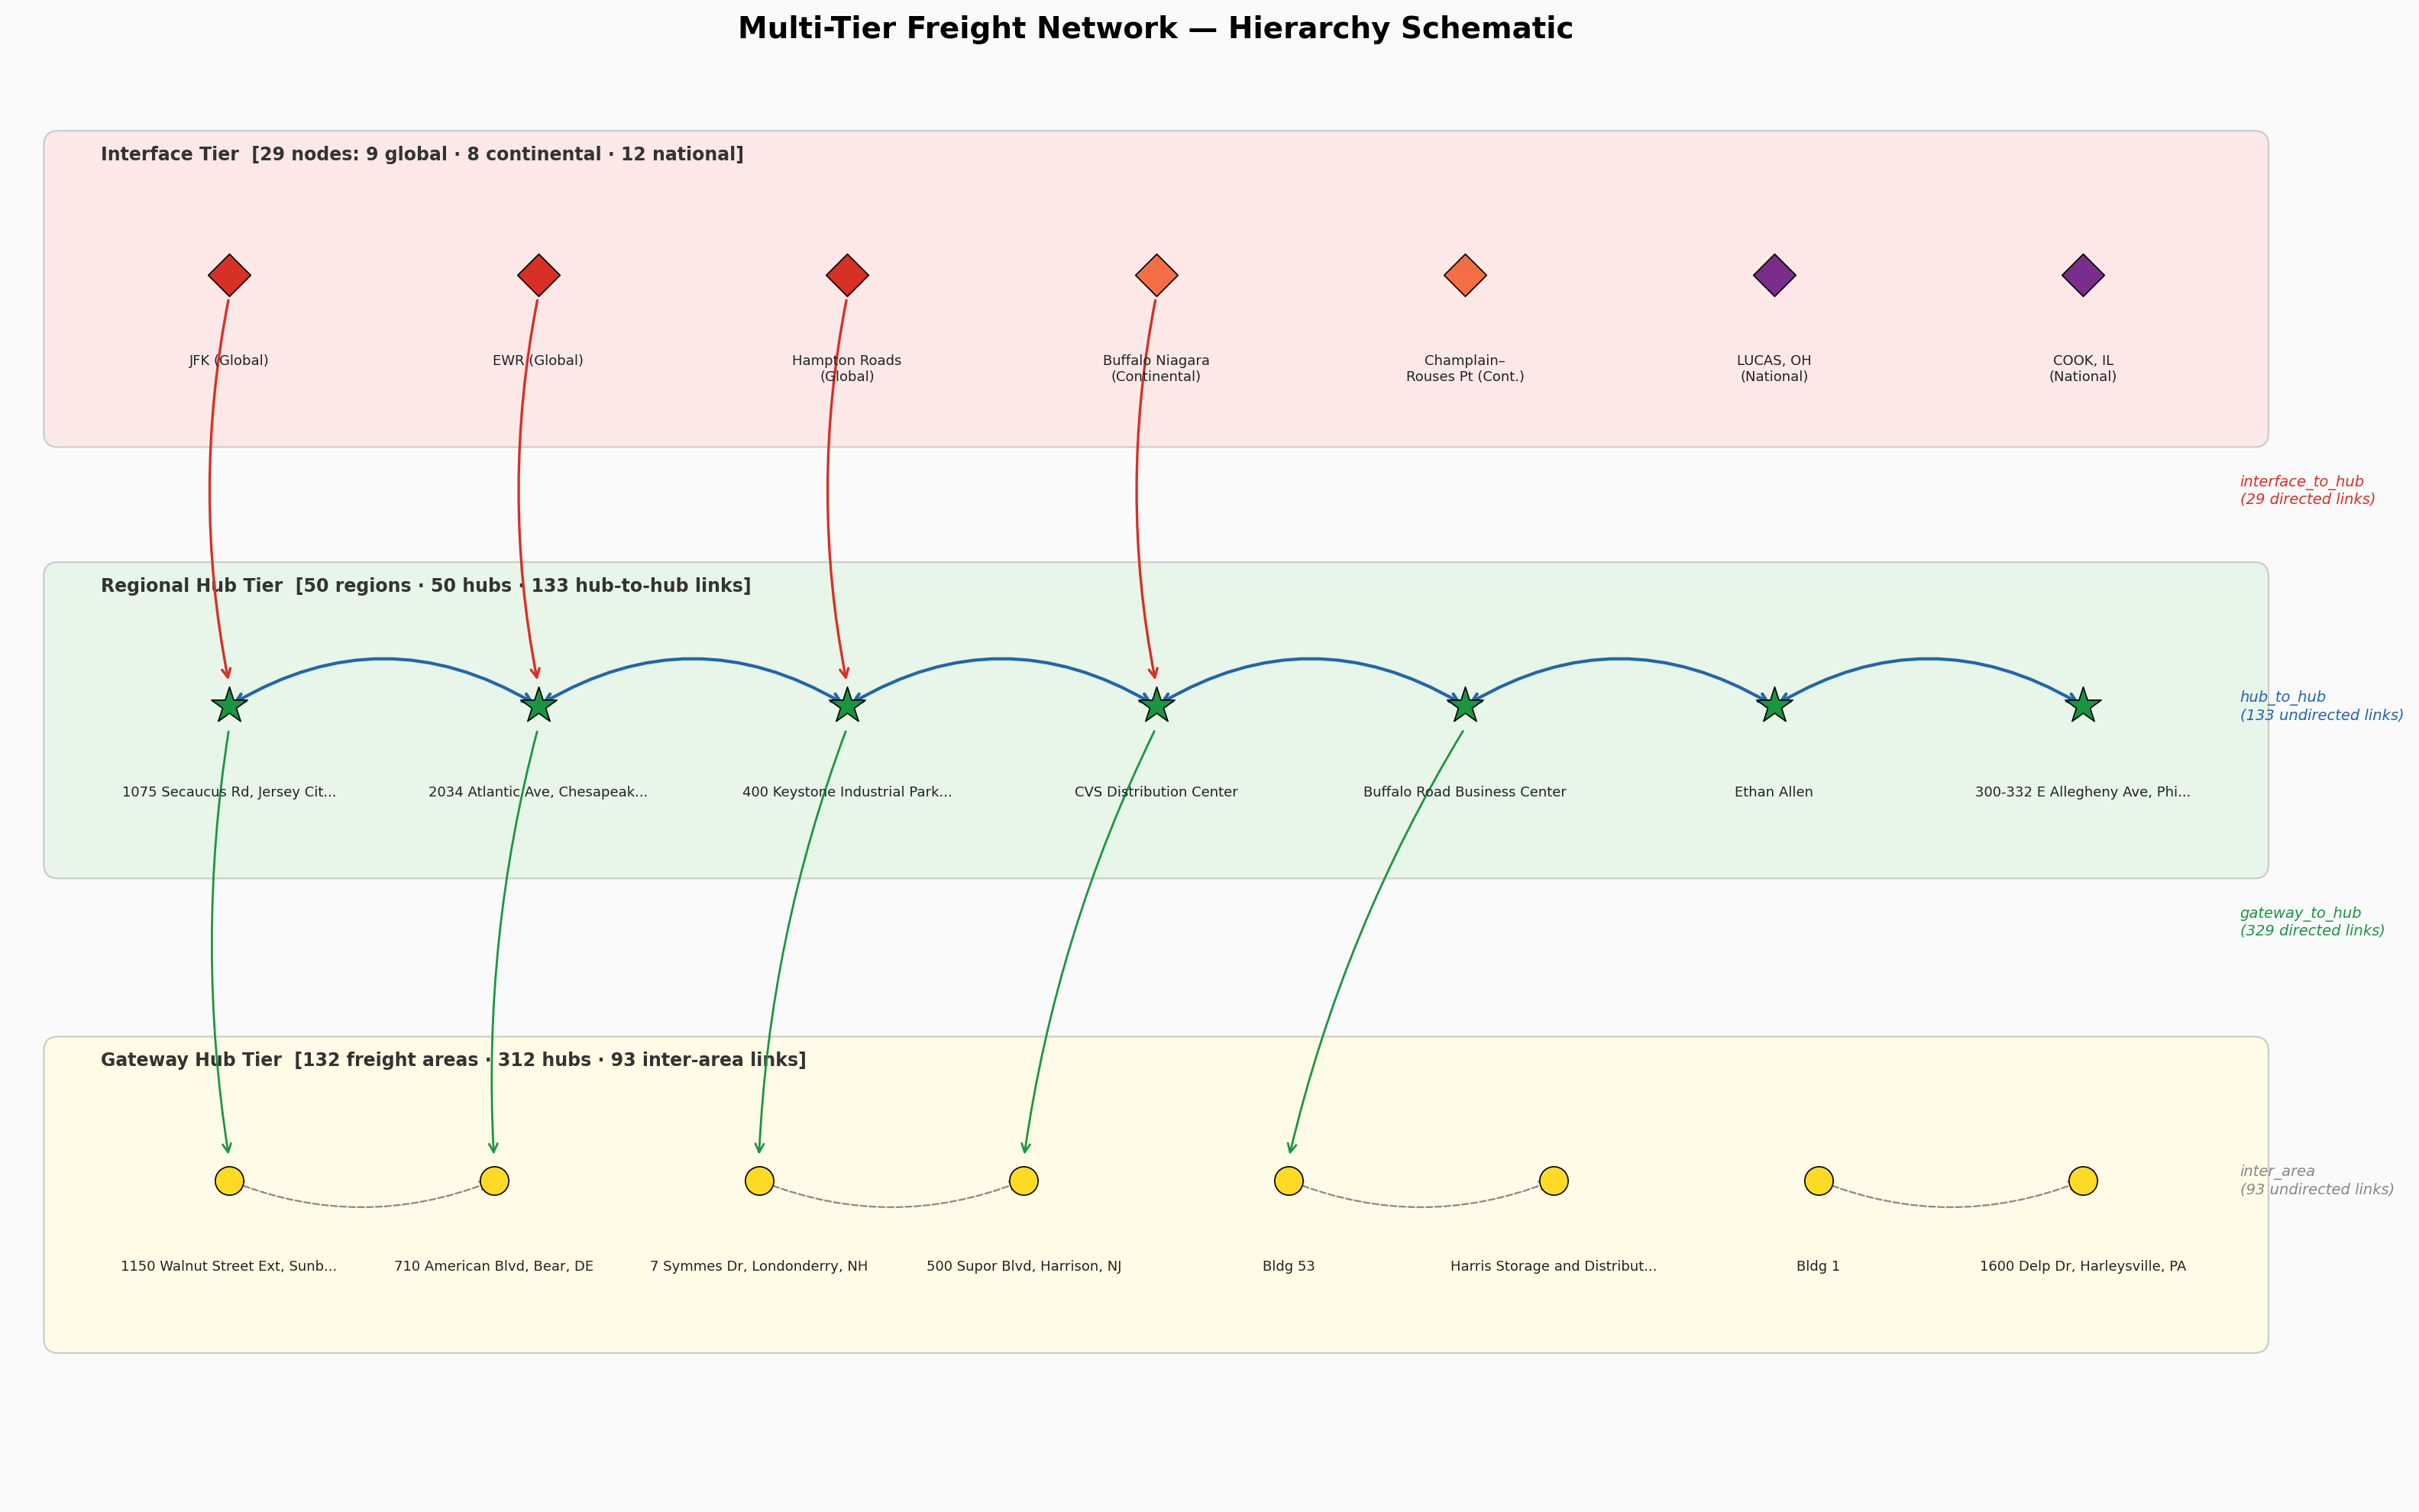
\includegraphics[width=0.95\textwidth]{figures/task7_hierarchy_schematic.png}
  \caption{Hierarchy schematic of the integrated three-tier design. The interface tier
    (29 nodes) feeds the regional hub tier (50 hubs connected by 133 hub-to-hub links),
    which in turn feeds the gateway tier (312 hubs serving 132 freight areas through
    329 gateway-to-hub links and 93 inter-area links). Only representative sample nodes
    are drawn, but the annotated counts reflect the full integrated network.}
  \label{fig:task7-schematic}
\end{figure}

The principal structural characteristic of the final design is therefore selective
density rather than uniform mesh connectivity. The regional backbone is sparse enough to
remain interpretable, but dense enough to keep all 50 hubs in a connected transfer
network. The gateway tier adds the fine-grained urban access that the regional tier
cannot provide on its own, while the interface tier localises the megaregion's external
exchanges to a tractable set of boundary anchors. This makes the Task~7 network a usable
bridge between the location models of Tasks~5--6 and the flow assignment calculations of
Task~8.
